\documentclass{acmart}
\usepackage{geometry}
\usepackage{amsmath}
\usepackage{graphicx}
\usepackage{float}
\usepackage{mathtools}
\begin{document}
\tableofcontents
\newpage
\section{Introduction}
With the ongoing evolution of wireless communication and localization technologies, locationbased services (LBSs) have been enjoying growing popularity in recent years. Starting from one of the earliest LBSs, the enhanced 911 (E911) system in the U.S. introduced in 1996 [5], LBSs have experienced remarkable development that continues to date. According to the Pew Research Center [108], 74\% of mobile users enjoyed LBSs in 2013, and the percentage increased to 90\% in 2015. In terms of time, mobile users spent approximately 900B hours using mobile applications (apps) in 2016, which represented an increase of 150B hours over the respective figure in 2015 [104]. According to the Berg Insight and PRNewswire [111], the worldwide revenue of LBSs increased to USD 10.86B in 2014 from USD 2.6B in 2009, stood at USD 15.04B in 2016 and is expected to reach USD 77.84B by 2021, expanding at a compound annual growth rate of 38.9\% during the forecast period. However, LBSs have also raised severe privacy concerns. While enjoying LBSs, users have to provide their location information involved in the LBS queries to the LBS server. It has been observed that the service provider may deliberately or inadvertently reveal sensitive location information embedded in LBS queries [131].
\begin{figure}[H]
    \centering
    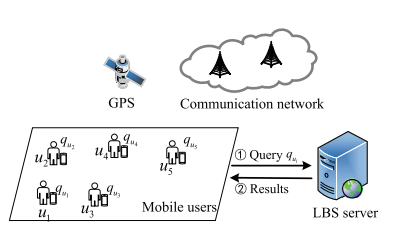
\includegraphics[width=100mm]{LBS Server.png}
    \caption{LBS Server}
    \label{1}
\end{figure}
\section{Preliminary notes}
In this section, we start with the network model of a typical LBS system (\ref{1}) and subsequently discuss location privacy concerns, the attack model, and the auxiliary knowledge of adversaries. Afterwards, we identify the objectives of location privacy preservation.
\\
Location Privacy-Preserving Mechanisms in Location-based Services:
\\
\begin{enumerate}
    \item Privacy Challenges in IoT;
    \item Challenges in Social Networks;
    \item Privacy Challenges in Machine Learning;
    \item The scope of knowledge;
    \item The intersection of LBS and social networks;
    \item Cloaking and Geo-indistinguishability.

\end{enumerate}
There are numerous sensing nodes in the sensing layer of IoT that can accurately sense the activity and state of users in the physical space in real time. Therefore, the Internet of Things has a large amount of side-channel data. Examples of such data include the Wi-Fi/Bluetooth connection records of a mobile device, the signal strength leaked while the device communicates, transmission activity in wireless networks, the data of electricity meters in a smart grid, and so on.

\subsection{Network Model of LBS}
The network model of LBSs consists of four entities, as shown in Figure (\ref{1}): mobile users, location positioning system, wireless communication networks, and the location-based services’ provider. In a typical LBS system, a mobile user (client) sends an LBS query to the LBS server over the
\begin{equation}
\label{f1}
    t^i = 
    \begin{cases}
    t^i_{\nu}, &\text{$W_i=1$}\\ 
    \frac{t^i_\nu-\nu p f^i \times \lambda_W}{i - \nu p f^i}, &\text{$W_i=0$, $I^i_{mean} \ge 128$}\\
    \frac{t^i_\nu-\nu p f^i \times (255-\lambda_W)}{i - \nu p f^i}, &\text{$W_i=0$, $I^i_{mean}$ < 128}\\
    \end{cases}
\end{equation}
Definition 1 (Differential Privacy). Assume a randomized algorithm A (the algorithm being randomized means that its output is not a fixed value for a particular input, but instead follows a certain distribution) and a positive real number.
\\
Entropy measures the degree of privacy protection from the perspective of the uncertainty in an attacker’s determination of a unique answer from all candidates. It has been frequently used with two subsets of LPPMs (\ref{f2}). The first definition is suitable for an anonymity framework [75] and applies to, e.g., cloaking, dummy locations, path confusion, and mix zone (2) mechanisms based on k-anonymity. In an anonymity framework, the entropy is computed as
\begin{equation}
\label{f2}
    t^i_\nu = 
    \begin{cases}
    t^i_\nu, &\text{$W^i=1$}\\
    {(1-\nu p f^i)t^i+\nu p f^i\times \lambda_W}, &\text{$W^i=0$, $I^i_{mean} \ge 128$}\\
    {(1-\nu p f^i)t^i+\nu p f^i\times(255 -\lambda_W)}, &\text{$W^i=0$, $I^i_{mean}$ < 128}
    \end{cases}
\end{equation}
To measure the data utility of the perturbed location, the expected distance between the released location and the actual location, which is also commonly referred to as quality of loss (\ref{f1}), can be a general utility metric independent of specific location-based applications and has been adopted as the standard by the community:
\begin{equation}
\label{f3}
  \prod _{LM}\left ( D,g(D)) \right )=\frac{1}{nr}\cdot \sum_{i=1}^{n}\sum_{j=1}^{r}\frac{\left | \bar{R}(j)) \right |  -1}{\left | A_{j} \right | -1}
\end{equation}

\subsection{Open Issues in Existing LPPMs}
\subsubsection{Performance. We discuss the following three aspects of performance in the context of the inherent tradeoff among location privacy, utility, and overhead in designing LPPMs}
\begin{description}
    
    \item[Quantification.]The development of LPPMs relies on the ability to theoretically quantify location privacy and loss of service quality.  However, current research mainly focuses on designing privacy preservation algorithms. Few studies aim at evaluating the efficiency of protection mechanisms in regard to privacy and utility [106, 116]. On the privacy side, an emerging option would be to improve robustness of LPPMs by jointly integrating two or more privacy notions based on their inherent limitations and complementary nature. 
    \item[Personalization.]Enabling personalized privacy protection for users is challenging but essential for users’ benefiting from location data. In practice, various users indeed have different requirements regarding location privacy and service utility. Even for the same user, requirements may vary for different types of services, locations, times, and environments.
    \item[Practicality.]The gap between theory and practice has been widening, and implementations of the proposed LPPMs in real-world applications remain underexplored. When LPPMs are being designed, it is necessary to take into account the availability of data and the efficiency of the system. 
    \item[Temporal and spatial correlations.]With the development of mobile computing and vehicle-to-everything (V2X) communications, the demand for mobile services (e.g., continuous LBSs) is growing.
    \item[Background knowledge correlations.]In an era of various applications and services being integrated, a fundamental challenge entails location privacy protection in the context of correlations among accessible multisource and cross-domain spatiotemporal data.

\end{description}
\subsubsection{LPPMS for continuous LBSS}
In contrast (\ref{f3}), policy-based privacy protection mechanisms face the highest risk of revealing private user information. The obfuscation-based and cooperation- and caching-based mechanisms perform comparably in this respect. Furthermore, we provide two insights. An individual location privacy-preserving mechanism uses the appropriate privacy metrics due to its distinct protection objectives and methodology.
\section{Research Opportunities Involving Emerging Technologies}
Utility As described in the previous subsection, the mainstream approach to preserving location privacy is location obfuscation (\ref{2}). Intuitively, the correctness of query results depends on the sanitized location (referred to as the released location) output by the LPPM rather than the user’s actual location.
\begin{figure}[H]
    \centering
    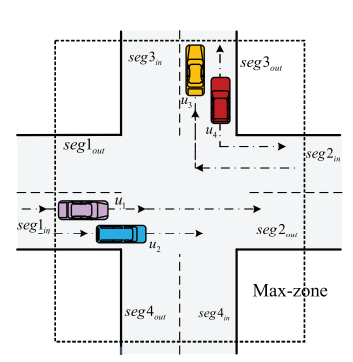
\includegraphics[width=50mm]{il.png}
    \caption{Illustration of the defenition of mix zones}
    \label{2}
\end{figure}
For a more intuitive understanding of utility degradation resulting from the obfuscation mechanism, we compare the service quality losses of the two perturbation mechanisms under the condition that both mechanisms guarantee the same level of geo-indistinguishability in our table(\ref{tab1})In summary, there are three main topics in the research of this technique, namely, reducing cache overhead, increasing the cache hit ratio, and improving the quantification of the level of location privacy and QoS. Another aspect that should be considered is reducing the costly communication overhead caused by this technique’s cooperative architecture.

\begin{table}[H]
\begin{tabular}{|p{2cm}|p{2cm}|p{2cm}|p{2cm}|p{2cm}|p{2cm}|} 
    \hline
    Category&Level of privacy&Utility&Computational overhead&Communication overhead&Storage overhead  \\
    \hline
    Privacy policy-based&Low&High&Low&Low&Low \\
    \hline
    Obfuscation-based&Medium&Medium&Medium&Medium&Low \\
    \hline
    Cryptography-based&High&High&High&High&Medium \\
    \hline
    Cooperation and caching-based&Medium&Medium&Low&High&High \\
    \hline
\end{tabular}
\caption{Comparative Evaluation}
\label{tab1}
\end{table}
\end{document}
